\lstset{language=Java}

\block{
	\section{Mobil kliens}

	\subsection{\mt{Áttekintés}{}}

	\p{\mt{%
		A mobil alkalmazás forrsás fájljai a \code{EasyInventoryMobile} mappában
		találhatóak, fejlesztésre pedig az Android Studió használható. A nyelvfájlokat a
		\code{langconvert.py} python program generálja. Az ikonok megegyeznek
		a webes frontend ikonjaival, viszont importálva lettek, így ikonmódosítás
		esetén érdemes újra importálni.
	}{}}
}

\block {
	\subsection{\mt{MainActivity osztály}{}}

	\p{\mt{%
			A program a \code{MainActivity} osztályban kezdődik, ami megjeleníti a bejelentkezési felületet, illetve amennyiben még nincs, engedélyt kér a hálózat használatához.
		}{}
		
		\lstinputlisting{generated/mobile.mainactivity.java}
	}
}

\block {
	\subsection{LoggedInActivity \mt{osztály}{}}

	\p{\mt{%
			A \code{LoggedInActivity} osztály megjeleníti a bejelentkezett felületet.
			A különböző fülek kódjai a saját \code{Fragment} osztájaikban vannak.
		}{}

		\lstinputlisting{generated/mobile.loggedinactivity.java}
	}
}

\block {
	\subsection{Worker \mt{osztály}{}}

	\p{\mt{%
			A \code{Worker} osztály a háttérben futó folyamatok kezeléséért felelős.
		}{}

		\lstinputlisting{generated/mobile.worker.java}
	}
}

\begin{landscape}
	\begin{figure}
		\centering
		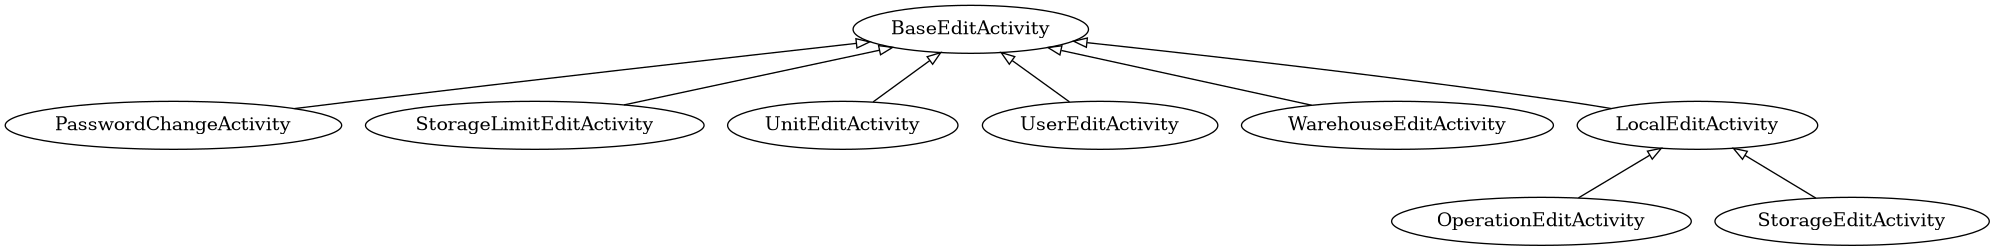
\includegraphics[width=\linewidth]{mobileclient.classes.png}
		\caption{\mt{Osztálydiagramm}{}}
	\end{figure}
\end{landscape}

\block {
	\subsection{BaseEditActivity \mt{osztály}{}}

	\p{\mt{%
			A \code{BaseEditActivity} absztrakt osztály a szerkesztési vagy hozzáadási tevékenységeknek a szülőosztálya.
			A \code{initUI} metódus feladata a felhasználói felület inicializálása.
			A \code{getItem} funkció feladata a bemeneti adat értelmezése.
			A \code{save} metódus feladata az adat mentése.
			A \code{readContext} funkció feladata a módosítandó adat kiolvasása a tevékenység adatokból.
		}{}

		\lstinputlisting{generated/mobile.baseeditactivity.java}
	}
}

\block {
	\subsection{LocalEditActivity \mt{osztály}{}}

	\p{\mt{%
			A \code{LocalEditActivity} absztrakt osztály a \code{BaseEditActivity} osztályt telephely bekéréssel egészíti ki.
			Ilyen tevékenység indításánál meg kell adni a kiválasztott telephely azonosítóját a \code{warehouse\_id} kulcsal.
		}{}

		\lstinputlisting{generated/mobile.localeditactivity.java}
	}
}

\begin{landscape}
	\begin{figure}
		\centering
		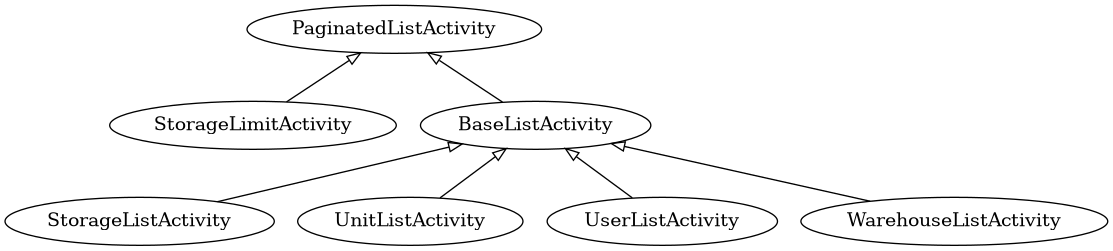
\includegraphics[width=\linewidth]{mobileclient.classes2.png}
		\caption{\mt{Osztálydiagramm}{}}
	\end{figure}
\end{landscape}

\block {
	\subsection{PaginatedListActivity \mt{osztály}{}}

	\p{\mt{%
			A \code{PaginatedListActivity} absztrakt osztály olyan tevékenységek szülőosztálya, amelyek lapozható listát mutatnak.
			A \code{load} funkció feladata, hogy a megadott paraméterek (keresési szüveg, kezdőpozíció, mennyiség, archivált-e) alapján betöltse az adatokat.
		}{}

		\lstinputlisting{generated/mobile.paginatedlistactivity.java}
	}
}

\block {
	\subsection{BaseListActivity \mt{osztály}{}}

	\p{\mt{%
			A \code{BaseListActivity} absztrakt osztály a kiválasztási felületek szülőosztálya.
			A \code{getNullDisplay} funkció feladata, hogy amennyiben a \code{load} funkció által visszaadott értékek között \code{null} érték is található, kicserélje azt a funkció visszatérési értékére.
		}{}

		\lstinputlisting{generated/mobile.baselistactivity.java}
	}
}

\begin{landscape}
	\begin{figure}
		\centering
		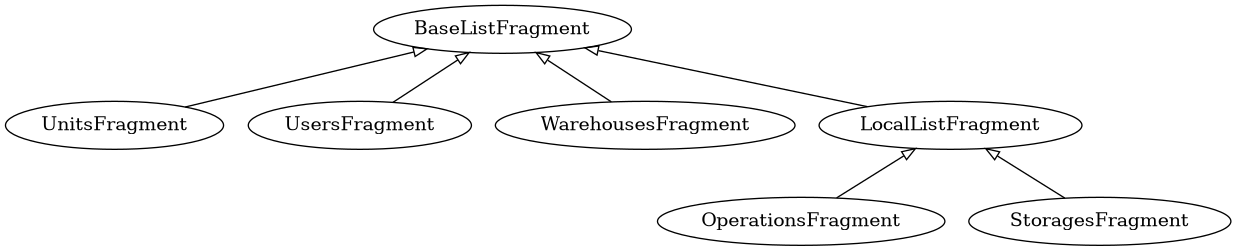
\includegraphics[width=\linewidth]{mobileclient.classes3.png}
		\caption{\mt{Osztálydiagramm}{}}
	\end{figure}
\end{landscape}

\block {
	\subsection{BaseListFragment \mt{osztály}{}}

	\p{\mt{%
			A \code{BaseListFragment} absztrakt osztály a lista \code{Fragment}-ek
szülőosztálya, melynek feladata a lapozás, a keresés, az újratöltés, a törlés és a szerkesztés indítása. A
\code{PaginatedListActivity} osztályhoz hasonlóan itt is megtalálható a \code{load} funkció. Az adat törlése a \code{delete} metódus feladata.
		}{}

		\lstinputlisting{generated/mobile.baselistfragment.java}
	}
}

\block {
	\subsection{LocalListFragment \mt{osztály}{}}

	\p{\mt{%
			A \code{LocalListFragment} absztrakt osztály a \code{BaseListFragment} osztályt telephely bekéréssel egészíti ki.
		}{}

		\lstinputlisting{generated/mobile.locallistfragment.java}
	}
}


\begin{landscape}
	\begin{figure}
		\centering
		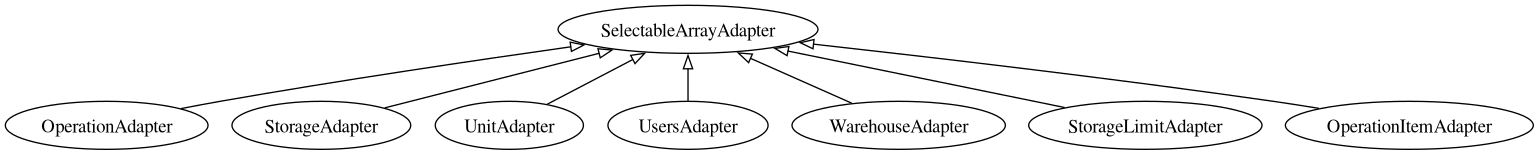
\includegraphics[width=\linewidth]{mobileclient.classes4.png}
		\caption{\mt{Osztálydiagramm}{}}
	\end{figure}
\end{landscape}

\block {
	\subsection{SelectableArrayAdapter \mt{osztály}{}}

	\p{\mt{%
			A \code{SelectableArrayAdapter} absztrakt osztály az \code{ArrayAdapter} osztály implementálását segíti kijelölhető listákra.
		}{}
	}
}

